\section{1D Model}

Let us look at the easiest possible model of the synaptic cleft; a 1D model. Assume the neurotransmitters diffuse along a line, released from the axon terminal and arriving at the dendritic spine. When the neurotransmitters attach and detach to the receptors, we model it as a total flux $J$ of neurotransmitters leaving or entering the domain. Further, we assume that when the neurotransmitters are within a small distance $\epsilon$ of the dendritic spine, they are close enough to react with the receptors.

The number of receptors on one membrane is R $\approx \gamma_R \cdot \pi r^2 \approx 152$, where $\gamma_R$ is the density of receptors and $r$ is the radius of the synaptic cleft \cite{task}. N $= 5000$ as before. Let $\Omega$ be the line between $0$ and $L$.

Now, look at the area near the dendritic spine. Let $\Omega_{\epsilon}$ be a small area close to $L$ with width $\epsilon$, see Figure \ref{fig:model_1d}. Let $\gamma_{N\epsilon}(t)$ be the density of neurotransmitters in $\Omega_{\epsilon}$, $\gamma_R$ the density of receptors in the area $\epsilon$, and $P^R(t)$ be the probability that one receptor is available. With reaction constants $k_1$ and $k_2$, the flux can be expressed as

\begin{align*}
J(t) = k_1 \gamma_{N\epsilon}(t) \gamma_R P^R(t) - k_2 \gamma_R (1-P^R(t)).
\end{align*}


\begin{figure}[ht]
        \centering
        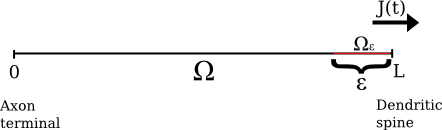
\includegraphics[clip=true,width=0.6\textwidth]{model_1d}
        \caption{Model of the synaptic cleft in one dimension}
        \label{fig:model_1d}
\end{figure}
\subsection{Initial values and boundary conditions}

Initial values:

\[ c(x,0) = \left\{ 
  \begin{array}{l l}
    \textrm{N} & \text{ if } x = 0\\
    0 & \text{ elsewhere}
  \end{array} \right.\]

Neumann boundary conditions:

\begin{align*}
c_x(0,t) &= 0, \\
c_x(L,t) &= J(t).
\end{align*}


The homogeneous Neumann boundary condition at $x = 0$ comes from the physical explanation that neurotransmitters cannot go back through the axon terminal.




\subsection{Scaling of variables}


We use the same scaling as in section 4 and replace in the unscaled diffusion equation (\ref{diffusion_unscaled}) such that

\begin{align*}
\frac{\textrm{N}}{T}\frac{\partial c}{\partial t} &= \kappa \frac{\textrm{N}}{L^2}\frac{\partial^2c}{\partial x^2} \Rightarrow
\frac{\partial c}{\partial t} = \eta \frac{\partial^2c}{\partial x^2}, & \eta = \kappa\frac{T}{L^2}.
\end{align*}

Using the values $L = 15 \cdot 10^{-9}$, $T = 10^{-3}$ and $\kappa = 0.3\cdot 10^{-12}$, we get the resulting value $\eta = 4/3$.




\subsection{Numerical scheme}

Using Crank-Nicholsons method, we obtain 

\begin{align*}
(1 - \frac{k}{2h^2} \delta^2_x)C^{n+1}_m = (1 + \frac{k}{2h^2} \delta^2_x) C_m^n,
\end{align*}

where $k$ and $h$ are the time and space steps, respectively. Adding Neumann boundary conditions to the system, we expand the numerical scheme to involve boundary points, and an additional term such that the resulting scheme becomes

\begin{align*}
\left(I - \frac{r}{2} A\right)C^{n+1} = \left(I + \frac{r}{2} A\right) C^n + \frac{k}{2}(d^n + d^{n+1}),
\end{align*}

where $r = \frac{k}{h^2}$,


\begin{align*}
A = 
\begin{pmatrix}
  -3/2h & 2h & -h/2 &  \\
  1 & -2 & 1 &  \\
  &  \ddots & \ddots & \ddots  \\
  &  & 1 & -2 & 1 \\
  &  & -3/2h & 2h & -1/2h 
\end{pmatrix} 
\textrm{, }
C = \begin{pmatrix}
C_0 \\
C_1 \\
\vdots \\
C_{M} \\
C_{M+1} 
\end{pmatrix}
\textrm{, }
d =
\begin{pmatrix}
0 \\
0 \\
\vdots \\
0 \\
J(t)
\end{pmatrix}.
\end{align*}

The result of this scheme is visualized in figure \ref{fig:model_1d_plot}. 


\begin{figure}[h!]
    \centering
    \begin{subfigure}[b]{0.45\textwidth}
        \centering
        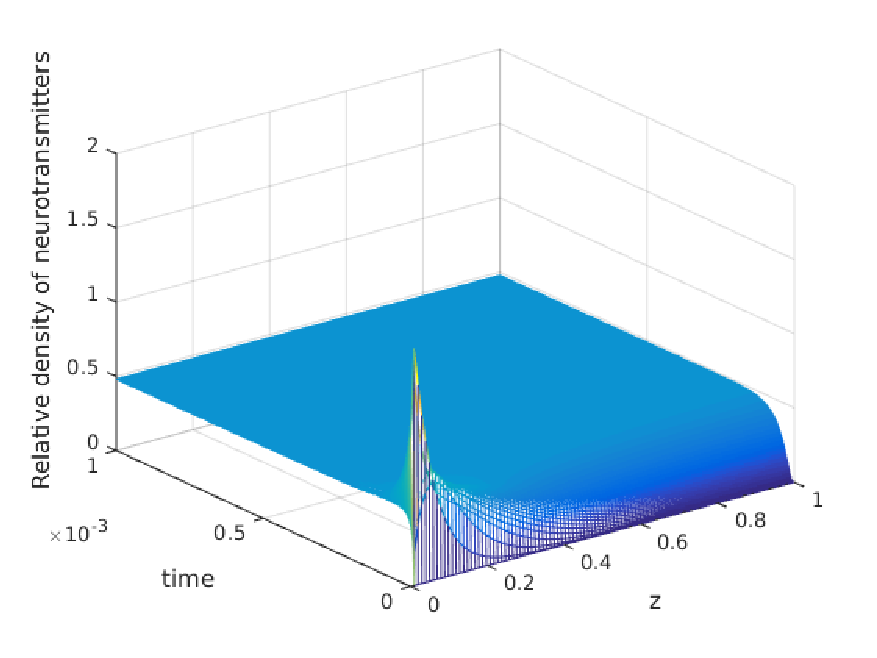
\includegraphics[width=\textwidth]{1dmodel_plot-crop}
        \caption{Distribution of neurotransmitters on a line over time. $k_1 = 10$, $k_2 = 1$, $\Delta t = 0.001$, $\Delta z = 0.01$.}
    \end{subfigure}%
    ~ 
    \begin{subfigure}[b]{0.45\textwidth}
        \centering
        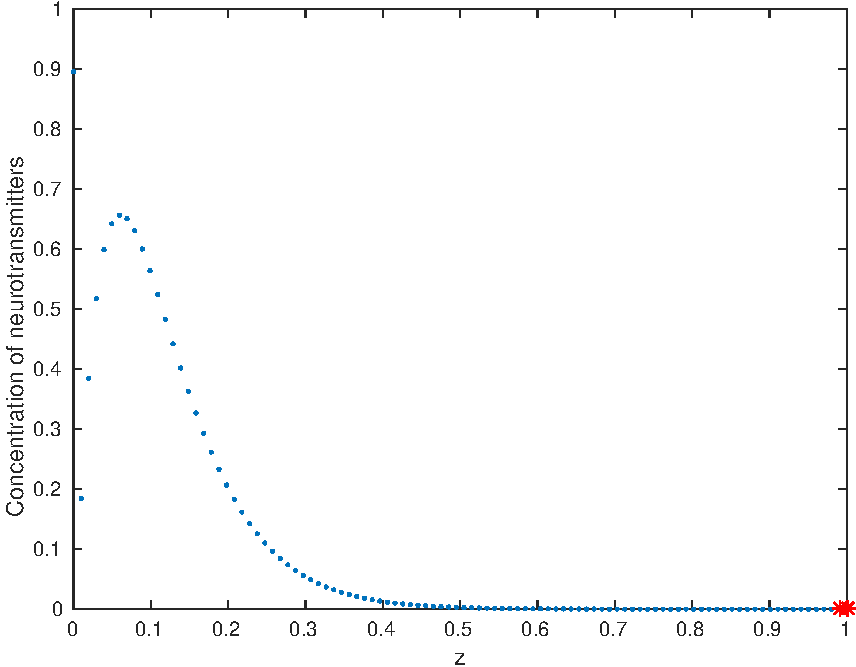
\includegraphics[width=\textwidth]{distribution_plot_1d-crop}
        \caption{Distribution of neurotransmitters on a line at a certain time. The red dots in the right corner marks $\Omega_{\epsilon}$.}
    \end{subfigure}
    \caption{Distribution of neurotransmitters on a line using the Matlab script $dim1.m$.}
    \label{fig:model_1d_plot}
\end{figure}